\chapter{Living and decaying roots as regulators of soil aggregation and organic matter formation---from the rhizosphere to the detritusphere}
\label{chap:manuscript5} % Label for potential cross-referencing (start page)

\begin{center}
    \textbf{\Large Manuscript 5}
  
    \vspace{0.3cm}
    \textit{Soil Biology and Biochemistry}\\
    \textit{DOI 10.1016/j.soilbio.2024.109503}
    
    \vspace{0.5cm}
    \begin{justify}
    Kristina Witzgall\textsuperscript{1}, Franziska Steiner\textsuperscript{1}, Benjamin D. Hesse\textsuperscript{2,3}, Nicolás Riveras-Muñoz\textsuperscript{4}, Victoria Rodríguez\textsuperscript{5}, Pedro Teixeira\textsuperscript{1}, Li, M.\textsuperscript{6}, Rómulo Oses\textsuperscript{7}, Oscar Seguel\textsuperscript{8}, Steffen Seitz\textsuperscript{4}, Dirk Wagner\textsuperscript{5,6}, Thomas Scholten\textsuperscript{4}, Franz Buegger\textsuperscript{9} Gerrit Angst\textsuperscript{7,11,12}, and Carsten W. Mueller\textsuperscript{1,13,14}
    \end{justify}
    \vspace{0.2cm}
  \end{center}
  
  \begin{scriptsize}
    \begin{justify}
        \textsuperscript{1}Soil Science, TUM School of Life Sciences, Technical University of Munich, Freising-Weihenstephan, Germany\\
        \textsuperscript{2}Land Surface Atmosphere Interactions -- AG Ecophysiology of Plants, TUM School of Life Sciences, Technical University of Munich, Freising-Weihenstephan, Germany\\
        \textsuperscript{3}Institute of Botany, Department of Integrative Biology and Biodiversity Research, University of Natural Resources and Life Sciences, Vienna, Austria\\
        \textsuperscript{4}Department of Geosciences, Soil Science and Geomorphology, University of T\"ubingen, T\"ubingen, Germany\\
        \textsuperscript{5}GFZ German Research Centre for Geosciences, Section Geomicrobiology, Potsdam, Germany\\
        \textsuperscript{6}Institute of Geosciences, University of Potsdam, Potsdam, Germany\\
        \textsuperscript{7}Biology Centre of the Czech Academy of Sciences, Institute of Soil Biology \& SoWa Research Infrastructure, \v{C}esk\'{e} Bud\v{e}jovice, Czech Republic\\
        \textsuperscript{8}Centro Regional de Investigaci\'{o}n y Desarrollo Sustentable de Atacama (CRIDESAT), Universidad de Atacama, Copiap\'{o}, Chile\\
        \textsuperscript{9}Facultad de Ciencias Agron\'{o}micas, Universidad de Chile, Santiago, Chile\\
        \textsuperscript{10}Research Unit Environmental Simulation, Helmholtz Zentrum M\"unchen (GmbH), German Research Center for Environmental Health, Neuherberg, Germany\\
        \textsuperscript{11}German Centre for Integrative Biodiversity Research Halle--Jena--Leipzig (iDiv), Leipzig, Germany\\
        \textsuperscript{12}Institute of Biology, Leipzig University, Leipzig, Germany\\
        \textsuperscript{13}Institute for Ecology, Chair of Soil Science, Technische Universit\"at Berlin, Berlin, Germany\\
        \textsuperscript{14}Department of Geosciences and Natural Resource Management, University of Copenhagen, Copenhagen, Denmark
    \end{justify}
  \end{scriptsize}
    
  \vspace{0.5cm}
  \begin{center}
    Received: 27 February 2024\\
    Received: 13 November 2023\\ 
    Received in revised form: 15 June 2024\\
    Accepted: 17 June 2024\\
    Available online: 18 June 2024
  \end{center}
  \cleardoublepage

\section*{Abstract}

In dryland ecosystems, typically characterized by sparse vegetation and nutrient scarcity, pioneer plants exert a critical role in the build-up of soil carbon (C). Continuous root-derived C inputs, including rhizodeposition and structural root litter, create hotspots of increased microbial activity and nutrient availability where biogeochemical processes, such as soil aggregation and the accumulation and stabilization of organic matter (OM), are promoted. Our study aims to disentangle the effects of root C inputs on soil aggregate formation, microbial community structures, and on the fate of OM—both before and after plant death, i.e., during the transition from rhizosphere to detritusphere. This was realized in a two-phase incubation approach, tracing the natural and undisturbed transition from growth to subsequent decomposition of a pioneer plant-root system (\textit{Helenium aromaticum}) in a semi-arid topsoil and subsoil. We quantified water-stable aggregates, investigated the fate and composition of OM separated into particulate and mineral-associated OM fractions (POM and MAOM), and observed successional changes in the root-associated microbiome. Our results underscore the significance of roots as vectors for macroaggregation within the rhizosphere in both topsoil and subsoil, associated with a particularly strong increase in fungal abundance in the subsoil. In topsoil, we identified root legacy effects in the detritusphere, as root-induced macroaggregation persisted after plant death, a phenomenon not observed in subsoil. These root legacy effects were accompanied by a clear succession towards Gram-positive bacteria, which appeared to outcompete fungi during root decomposition. The increased availability of decaying litter surfaces further facilitated the protection of particulate OM via the occlusion into aggregates. Overall, to gain a holistic understanding of plant-microbe-soil interactions, we emphasize the need for more studies that span over the full temporal dimension from living to dying plants in intact soil systems.

\section{Introduction}

In dryland ecosystems, typically characterized by sparse vegetation and nutrient scarcity, pioneer plants exert a critical role in the build-up of soil carbon (C). Continuous root-derived C inputs, including rhizodeposition and structural root litter, create hotspots of increased microbial activity and nutrient availability where biogeochemical processes, such as soil aggregation and the accumulation and stabilization of organic matter (OM), are promoted. Our study aims to disentangle the effects of root C inputs on soil aggregate formation, microbial community structures, and on the fate of OM---both before and after plant death, i.e., during the transition from rhizosphere to detritusphere. This was realized in a two-phase incubation approach, tracing the natural and undisturbed transition from growth to subsequent decomposition of a pioneer plant-root system (\textit{Helenium aromaticum}) in a semi-arid topsoil and subsoil. We quantified water-stable aggregates, investigated the fate and composition of OM separated into particulate and mineral-associated OM fractions (POM and MAOM), and observed successional changes in the root-associated microbiome. Our results underscore the significance of roots as vectors for macroaggregation within the rhizosphere in both topsoil and subsoil, associated with a particularly strong increase in fungal abundance in the subsoil. In topsoil, we identified root legacy effects in the detritusphere, as root-induced macroaggregation persisted after plant death, a phenomenon not observed in subsoil. These root legacy effects were accompanied by a clear succession towards Gram-positive bacteria, which appeared to outcompete fungi during root decomposition. The increased availability of decaying litter surfaces further facilitated the protection of particulate OM via the occlusion into aggregates. Overall, to gain a holistic understanding of plant-microbe-soil interactions, we emphasize the need for more studies that span over the full temporal dimension from living to dying plants in intact soil systems.

A critical aspect of the plant-associated contribution to these soil processes occurs at the root-soil interface, i.e., within the rhizosphere. As plants grow, their roots physically alter soil minerals, and root-associated microorganisms release weathering agents (e.g., organic acids; \citeauthor{Uroz2009}, \citeyear{Uroz2009}) that mobilize essential soil nutrients \citep{Gregory2022}. 
In addition, the release of rhizodeposits at the root-soil interface represents a major pathway for the build-up of rather persistent mineral-associated OM (MAOM) in soil \citep{Sokol2019, Villarino2021}. Moreover, the increased abundance of labile C in the rhizosphere stimulates the growth and activity of microorganisms. This in turn drives the formation of aggregates via microbially derived binding agents (i.e., extracellular polymeric substances; EPS) or via the enmeshment facilitated by fungal hyphae \citep{Chenu2011, Costa2018}. In addition, root exudates (e.g., root mucilage or polysaccharide exudates) can either adhere directly to mineral surfaces or function as glue-like binding agents, binding soil particles together, forming MAOM \citep{Roetzer2023} and driving soil aggregation \citep{Baumert2018}. As such, roots substantially shape the chemical, physical, and biological nature of the soil at the root-soil interface, and the rhizosphere is widely recognized as a dynamic system in both space and time \citep{Jones2009, Hinsinger2009, Kuzyakov2019}. However, relatively little is known about the temporal changes in processes occurring in the rhizosphere, as well as potential long-term effects of the living root system that may persist beyond the lifetime of the roots \citep{Oliver2021}. These effects, so-called 'root legacy effects', might have implications for soil physical, chemical, and biological parameters that can remain in the soil after plant death and thus shape the subsequent detritusphere \citep{Wurst2015}.

As the rhizosphere transitions to a root detritusphere and the release of root exudates ceases, the soil environment in the vicinity of the decaying root changes. In the early stages of the rhizosphere-detritusphere transition, the concentration of easily available and water-soluble compounds from the decaying root litter is still high \citep{Cotrufo2015}. In addition, the microbial community is influenced by the labile C inputs remaining from the rhizosphere, which is thought to accelerate the decomposition and transformation of root litter into soil OM (SOM) in the developing detritusphere \citep{Wang2014}. Over time, bioavailable compounds are gradually depleted and replaced by complex and slowly decomposing compounds. This has implications for the microbial community composition, driving a succession of microbial communities from microorganisms that rely on root exudates for energy to those involved in the decomposition of more recalcitrant litter compounds \citep{Berg2008, Theuerl2010, Poll2010}. This can be reflected in the composition of the bacterial community, as a common indicator of decreasing availability of labile C sources is the relative increase in Gram-positive (Gram+) bacteria compared to Gram-negative (Gram-) bacteria \citep{Fanin2019}. In the resulting detritusphere, the degradation of litter residues constitutes a hotspot for SOM formation, similar to the rhizosphere. This occurs by a variety of mechanisms, including the direct formation of MAOM achieved by the association of microbial-derived OM to mineral surfaces \citep{Kopittke2020, Vidal2021}, or via the occlusion of particulate OM (POM) within aggregates directly at the surface of decaying litter \citep{Witzgall2021}.

The rhizosphere and the detritusphere both represent hotspots for root-microbe-soil interactions, driving the formation of soil structures and the development and preservation of SOM---not only in the near-root environment, but also at larger scales \citep{Richter2007}. Similarly, these effects also extend from surface soils into the subsoil, where roots constitute a major---if not the only---source of C into the deeper soil horizons otherwise characterized by low OM contents, heterogeneously distributed C, and low microbial activity \citep{Rasse2005, Chabbi2009}. Previous studies demonstrate how the importance of root C inputs for OM formation \citep{Angst2018}, long-term C persistence \citep{Eusterhues2003}, and macroaggregation \citep{Baumert2018} increase with increasing soil depth. In addition, \citet{Peixoto2020} show enhanced stabilization of root-derived C inputs in subsoils compared to in topsoil, and \citet{Wang2014} found increased incorporation rates of lignin-rich root derivatives into macroaggregates in subsoils. In semiarid shrub and grasslands, the deeper soil layers account for more than half of the total SOC stock across the soil profile \citep{Jobbagy2001}, and the subsoil C stock is expected to be less vulnerable to changes in climate and land management compared to semiarid surface soils \citep{Albaladejo2013}. Despite the significance of roots as a primary C source, the fluxes and stabilization mechanisms of root C in subsoils remain unknown \citep{Gregory2022}, particularly so in the context of dryland ecosystems.

Here, we examine the interactions of root OM inputs with soil aggregate formation and the fate of SOM into POM and MAOM at the root-soil interface in living and decaying root systems of a semiarid top- and subsoil. In order to simulate these processes during the early stages of soil formation, two incubation phases were conducted, mimicking the natural growth process of a pioneer perennial herbaceous plant species (\textit{Helenium aromaticum} (Hook.) L. H. Bailey); the first phase with living plants ('rhizosphere phase') with rhizodeposits as the main C input, followed by a decomposition phase ('detritusphere phase'), with plant and root litter as the main C input source. While numerous studies have contributed to our understanding of biogeochemical and microbial processes in both the rhizosphere and detritusphere (e.g., \citep{Poll2008}; \citep{Marschner2012}; \citep{Tian2013}; \citep{Vidal2021}), these systems are often studied separately. This means that the succession from a living to a decaying root system is not included, nor are the potential legacy effects from the rhizosphere that could influence processes in the developing detritusphere \citep{Wurst2015}. Furthermore, potential interactions between rhizodeposits and root litter as the two main root C inputs to SOM are unknown. To address this research gap, we employed an experimental design in which the transition from rhizosphere to root detritusphere, as well as the establishment of the root-associated microbiome, remained undisturbed. Replicates were sampled at two time points, at the end of the rhizosphere and detritusphere phase, after which the distribution of water-stable aggregates and their contribution to the total C and N pool were quantified by wet-sieving. The fate and chemical composition (C, N, \textsuperscript{13}C and \textsuperscript{15}N) of OM in POM (free POM (fPOM), occluded POM (oPOM and oPOM<\SI{20}{\micro\metre})) and MAOM was determined by density fractionation and \textsuperscript{13}C CP-MAS NMR. Lignin-derived phenols were extracted from plant and root biomass, and the structure of root-associated microbial communities in the rhizosphere and detritusphere was characterized by phospholipid fatty acid (PLFA) extractions. We hypothesized that roots would promote the formation of water-stable macroaggregates in both topsoil and subsoil, and that root-induced aggregation would remain after plant death in the detritusphere as root legacy effects. We assumed that microbial abundance would increase in the rhizosphere, particularly in the C-poor subsoil, due to the increased abundance of labile C around the roots. We further hypothesized that the transition to the detritusphere, as labile C compounds are depleted and replaced by more complex litter-derived compounds, would induce a succession in the root-associated microbiome, specifically towards increasing Gram-positive bacterial abundance.

\section{Material and methods}
\subsection{Study site and soil sampling}

Soil was sampled from five subplots on south-facing top slopes within the Santa Gracia Natural Reserve, located in the Coquimbo Region in Chile (\ang{29;44;26.3}S, \ang{71;09;01.2}W) with mean annual precipitation of \SI{89}{\milli\metre\,\year^{-1}} and mean annual air temperature of \SI{13.7}{\degreeCelsius} \citep{MinisterioObrasPublicas2017}. All five subplots were classified as Cambisol according to the WRB \citep{IUSS2015}. Vegetation was dominated by shrubs (\SIrange{30}{40}{\percent} coverage; including \textit{Proustia cuneifolia}, \textit{Balbisia peduncularis}, \textit{Cordia decandra} and \textit{Baccharis paniculatum}), classified as 'Interior Mediterranean desert scrub' \citep{Luebert2006}, and heavily disturbed by grazing animals \citep{Oeser2018}. The sampling site was selected as a suitable representation of an initial dryland soil with low vegetation cover, low organic C content, shallow and weakly structured A horizon \citep{Bernhard2018}. Topsoil and subsoil material was collected and sieved (\SI{< 2}{\milli\metre}) from the profile walls of A and B horizons (\SIrange{0}{3}{\centi\metre} and \SIrange{5}{30}{\centi\metre}, respectively), representing soils at different stages of development. This allowed us to directly compare topsoil and subsoil, but also to use the subsoil as a model system for initial soil formation via plant-soil interactions in a saprolitic material.

\subsection{Soil preparation and incubation setup}

The topsoil and subsoil material from the five subplots was homogenized and cleared of plant residues and seeds to prevent unwanted germination during incubation. The two soil materials (topsoil and subsoil) were weighed separately into pots (\SI{350}{\centi\metre\cubed}) aiming to resemble bulk density according to field conditions (\SIrange{1.6}{1.7}{\gram\per\centi\metre\cubed}; \citeauthor{Bernhard2018}, \citeyear{Bernhard2018}). Pre-germinated seeds (\textit{Helenium aromaticum} (Hook.) L. H. Bailey) were sown on half of the pots, while the other half was left free of plants and hereafter referred to as controls. After the initial incubation period of 70 days under greenhouse conditions ('rhizosphere phase'), half of the samples were harvested, while the remaining half were placed in complete darkness and incubated at room temperature for 100 days ('detritusphere phase'). The samples were left completely undisturbed during decomposition, meaning that above-ground biomass was left to decompose on the soil surface. During both incubation phases, the samples received \SI{6}{\milli\liter} of rainwater per day, without correcting for potential differences in soil moisture, e.g. due to differences in plant water use between treatments.

After incubation, the plants were cut just above the soil surface and the roots were separated from the bulk soil. To minimize artifact effects of biocrust on the soil surface, the top \SIrange{0}{1}{\centi\metre} of all samples was discarded \citep{Weber2022}. The soil sticking to the roots was collected separately and hereafter referred to as 'root-adhering soil'. Since the pots were thoroughly rooted, the remaining soil in the pots was defined as 'rhizosphere soil'. During the detritusphere phase, there was not enough soil adhering to the decaying roots to sample separately, meaning that all the soil in the pots were collected as 'detritusphere soil' from this phase. After incubation, replicate samples were combined in pairs (two by two) to form composite replicates. As such, there were initially 12 replicates per treatment during the incubation phases (48 pots in total), which later resulted in 6 composite replicates for each treatment for subsequent analyses. After harvest, plant and root samples were immediately frozen in liquid N. A homogenized aliquot of each soil sample was freeze-dried and stored at \SI{-20}{\degreeCelsius} for later microbial analyses (section 2.3). The remaining bulk soil material was air-dried at room temperature. Plant and root samples were analyzed for C, N, \textsuperscript{13}C, \textsuperscript{15}N (section 2.6), and lignin-derived phenols were extracted (section 2.8). Basic soil parameters (pH and electrical conductivity) were determined for soil material before and after each incubation period, and the gravimetric water content was determined for incubated samples.

\subsection{Phospholipid fatty acid analyses}

Phospholipid fatty acid (PLFA) patterns were recorded as reported by \citet{Frostegard1993} with adjustments according to the modified method by \citet{Kramer2013}. Briefly, \SI{4}{\gram} topsoil and \SI{12}{\gram} subsoil were vortexed with Bligh \& Dyer solution [methanol, chloroform, citrate buffer (pH=4 \(\pm\)0.1), 2:1:0.8, v/v/v] to extract lipids from the soil. Phospholipids were separated from neutral lipids and glycolipids by solid phase extraction on silica tubes (\SI{0.5}{\gram} SiOH, Bond Elut SI, Agilent Technologies) and later evaporated at \SI{40}{\degreeCelsius} under a stream of N\textsubscript{2} (\(\sim\)\SI{100}{bar}). The separated PLFAs were turned into fatty acid methyl esters (FAMEs) via alkaline methanolysis and later resolved in isooctane, from which the concentration of FAMEs was quantified via gas chromatography coupled to a flame ionization detector (Thermo Scientific Trace 1310, Waltham, MA, USA). The gas chromatograph was equipped with a ZB-5HT fused silica capillary column (\SI{60}{\metre}, 0.25 I.D., \SI{0.25}{\micro\metre} film thickness; Zebron Capillary GC column, Inforno\textsuperscript{TM}). The following FAMEs were selected for quantification; bacteria: C15:0 and C17:0, including Gram-positive bacteria: i15:0, a15:0, i16:0 and i17:0 \citep{OLeary1988} and Gram-negative bacteria: 16:1\(\omega\)7, cy17:0 and cy19:0 \citep{Phillips2002}, fungi: 18:2\(\omega\)6 and 18:1\(\omega\)9 and unspecified microorganisms: C14:0, C16:0, 18:1\(\omega\)7, C18:0 and C20:0. These markers were used to calculate fungi to bacteria (fungi:bacteria) and Gram+:Gram- ratios. 
The quantification and classification of PLFAs were based on non-adecanoic acid methyl ester (19:0) as the internal standard.

\subsection{Aggregate fractionation}

To separate water-stable aggregates, \SI{5}{\gram} air-dried aliquots of bulk soil were rewetted with deionized water for \SI{30}{\minute} and placed on a sieve tower (mesh size: \num{250} and \SI{53}{\micro\metre}, diameter: \SI{100}{\milli\metre}) in a beaker containing \SI{2}{\liter} deionized water. Aggregates were separated into macroaggregates (\SIrange{250}{2000}{\micro\metre}), large microaggregates (\SIrange{53}{250}{\micro\metre}) and small microaggregates including silt and clay particles (\SI{< 53}{\micro\metre}) by gentle up and downward movement (\SI{2}{\centi\metre}) repeated for 130 cycles, while the soil material was completely submerged in water \citep{Baumert2018}. The small microaggregate fraction was retained on a \SI{0.45}{\micro\metre} filter, and all samples were finally dried at \SI{40}{\degreeCelsius}. On average, \SI{99.3 \pm 0.4}{\percent} of the soil material was recovered from the fractionation process.

\subsection{Density and particle size fractionation}

Bulk soil was separated into five distinct OM fractions using a combined density and particle size fractionation approach according to \citet{Mueller2009}. Briefly, \SI{30}{\gram} of air-dried soil (\SI{50}{\gram} for subsoil) was saturated with a polytungstate solution (\ce{Na6[H2W12O40]}) at a density of \SI{1.8}{\gram\per\centi\metre\cubed} for \SI{12}{\hour}, after which free-floating particulate OM (fPOM) was separated from the bulk using a vacuum pump. Ultrasonic dispersion (Bandelin, Sonoplus HD 2200; \SI{440}{\joule\per\milli\liter}) was used to release occluded POM (oPOM) from aggregated soil structures, and the fraction was later sieved at \SI{20}{\micro\metre} to yield oPOM and oPOM $<$\SI{20}{\micro\metre} (oPOM\textsubscript{small}). Finally, the remaining mineral material was separated into two mineral fractions: MAOM$>$\SI{63}{\micro\metre} and MAOM<\SI{63}{\micro\metre}. All fractions were washed with deionized water, pressure filtered (\SI{0.22}{\micro\metre}) below an electrical conductivity of $<$\SI{5}{\micro\siemens\per\centi\metre}, ground and freeze-dried before elemental analysis.

\subsection{Carbon and nitrogen measurements of bulk soil and fractions}

Plant and root biomass, root-adhering soil, and OM fractions were analyzed for C, N, \textsuperscript{13}C, and \textsuperscript{15}N (Delta V Advantage, Thermo Fisher, Dreieich, Germany) coupled with an elemental analyzer (Euro EA, Eurovector, Milano, Italy). The aggregate size fractions were analyzed for C and N (EuroVector EuroEA3000 Elemental Analyzer). The presence of \ce{CaCO3} was examined through gas volumetric analysis (Scheibler Calcimeter; Eijkelkamp, Giesbeek, Netherlands) in which HCl was added to the soil and the gas pressure of the resulting \ce{CO2} was used to calculate \ce{CaCO3} contents. No reaction could be determined and the presence of \ce{CaCO3} could thereby be ruled out, meaning that total C contents were considered equal to total OC contents.

\subsection{\textsuperscript{13}C nuclear magnetic resonance spectroscopy}

The chemical composition of below- and aboveground plant material and POM fractions was determined via solid state \textsuperscript{13}C CP-MAS NMR spectroscopy (Bruker DSX 200, Bruker BioSpin GmbH, Karlsruhe, Germany). The samples, placed in \SI{7}{\milli\metre} zirconium dioxide rotors, were spun at \SI{6.8}{\kilo\hertz} with an acquisition time of \SI{0.01024}{\second} and a delay time of \SI{1.0}{\second} for plant material and \SI{0.4}{\second} for POM fractions. After a manual baseline correction, the recorded \textsuperscript{13}C spectra were quantified according to \citet{Mueller2009} with the following chemical shift regions: alkyl C ($-$10--45\,ppm), O alkyl C (45--110\,ppm), aromatic C (110--160\,ppm), and carbonyl/carboxyl C (160--220\,ppm). Further, we computed the alkyl C/O alkyl C ratio ($-$10--45/45--110\,ppm) according to \citet{Baldock1997} as well as the O alkyl C/methoxyl C and N alkyl C ratio (70--75/52--57\,ppm) according to \citet{Bonanomi2013} as a proxy for the stage of decomposition. Lastly, the spectra were modeled via the molecular mixing model \citep{Nelson2005, Prater2020} to compute the relative contribution of carbohydrates, proteins, lignins, lipids, and carbonyls. For the model, the chemical shift regions 0--45, 45--60, 60--95, 95--110, 100--145, 145--165, and 165--215\,ppm were applied.

\subsection{Lignin extraction}

Lignin-derived phenols were extracted from plant and root samples via cupric oxide (CuO) oxidation according to \citet{Angst2017}. Samples containing at least \SI{5}{\milli\gram} C were weighed into pressure digestion vessels with \SI{50}{\milli\gram} ammonium iron (II) sulfate hexahydrate and \SI{300}{\milli\gram} CuO, saturated with \SI{2}{M} NaOH and shaken at \SI{155}{\degreeCelsius} for \SI{3}{\hour}. The NaOH was separated by centrifugation and acidified with \SI{6}{M} HCl, and the remaining solution was extracted with ethyl acetate, filtered over \ce{Na2SO4}, and dried under N\textsubscript{2}. The sum of vanillyl, syringyl, and cinnamyl units (VSC) was used as an indicator for total lignin contents. The ratio between lignin-derived phenolic acids and their corresponding aldehydes was computed for vanillyl ((Ac/Al)\textsubscript{V}) as well as combined for all units (Ac/Al).

\subsection{Statistics}

We tested all parameters for homoscedasticity using Levene's test and the residuals of each model were tested for Normality using QQ-Plots and the Shapiro-Wilk test. In cases where the assumption of normality or homoscedasticity was not met, the data was appropriately transformed. To evaluate differences between the data presented in Table \ref{tab:M5-T1}, we conducted a one-way analysis of variance (ANOVA) with Tukey's honestly significant differences (HSD) as a post-hoc test. The remaining data was analyzed using mixed-effect models (package: \texttt{nlme}) using soil material (topsoil vs subsoil) and phase (rhizosphere phase vs detritusphere phase) as fixed factors and the ID as a random effect. All statistical testing was conducted in R (version 4.2.1; \citeauthor{RCoreTeam2008}, \citeyear{RCoreTeam2008}) using RStudio (Version 2022.07.2, R Core Team, Vienna, Austria; \citeauthor{RStudioTeam2015}, \citeyear{RStudioTeam2015}). Further, data shown in text and tables are given as the mean values and standard deviations.



\begin{table}[htbp]
  \centering
  \scriptsize
  \caption{Elemental and isotopic composition of above- and belowground biomass. Relative amounts of carbohydrates, proteins, lignin, lipids, and carbonyls from two incubation phases in topsoil and subsoil. Asterisks denote significance ($\bullet$ $p < 0.1$, *$p < 0.05$, **$p < 0.01$, ***$p < 0.001$).}
  \begin{tabular}{llcccc}
  \toprule
  \textbf{Category} & \textbf{Property} & Rhizo Above & Rhizo Below & Detri Above & Detri Below \\
  \midrule
  \multicolumn{6}{c}{\textbf{Topsoil}} \\
  \midrule
  \multirow{8}{*}{Basic properties} & C (mg g$^{-1}$) & 4.06 $\pm$ 0.20 & 3.70 $\pm$ 0.08 & 3.49 $\pm$ 0.47 & 3.97 $\pm$ 0.74 \\
  & N (mg g$^{-1}$) & 0.17 $\pm$ 0.05** & 0.11 $\pm$ 0.02** & 0.25 $\pm$ 0.06** & 0.11 $\pm$ 0.02** \\
  & C:N & 25.61 $\pm$ 7.77** & 34.43 $\pm$ 3.43** & 14.67 $\pm$ 3.99*** & 37.26 $\pm$ 8.89 \\
  & Biomass (g) & 0.47 $\pm$ 0.17*** & 0.44 $\pm$ 0.13*** & 0.11 $\pm$ 0.07*** & 0.03 $\pm$ 0.02*** \\
  & Total biomass (g) & 0.90 $\pm$ 0.22*** & 0.13 $\pm$ 0.09*** & 0.54 $\pm$ 0.11*** & 0.05 $\pm$ 0.07*** \\
  & Root:shoot & 1.07 $\pm$ 0.48** & 0.32 $\pm$ 0.20** & 1.27 $\pm$ 0.37 & 0.24 $\pm$ n.a. \\
  & C (mg) & 1.91 $\pm$ 0.78*** & 1.62 $\pm$ 0.51*** & 0.38 $\pm$ 0.29*** & 0.12 $\pm$ 0.09*** \\
  & N (mg) & 0.07 $\pm$ 0.02*** & 0.05 $\pm$ 0.01*** & 0.03 $\pm$ 0.02*** & 0.00 $\pm$ 0.01*** \\
  & $\delta^{15}$N ($\permil$ air N$_2$) & 4.96 $\pm$ 0.78 & 4.14 $\pm$ 0.59$^{\bullet}$ & 4.29 $\pm$ 0.71 & 3.22 $\pm$ 0.81$^{\bullet}$ \\
  & $\delta^{13}$C ($\permil$ V-PDB) & -29.84 $\pm$ 0.78 & -28.68 $\pm$ 0.51 & -29.46 $\pm$ 1.34 & -29.50 $\pm$ 1.01 \\
  \midrule
  \textbf{Relative contents} & Carbohydrate$_{\text{NMR}}$ & 53.68 $\pm$ 7.07$^{\bullet}$ & 57.69 $\pm$ 2.31** & 42.67 $\pm$ 8.17$^{\bullet}$ & 44.60 $\pm$ 8.41** \\
  & Protein$_{\text{NMR}}$ & 10.76 $\pm$ 3.47** & 7.46 $\pm$ 1.36 & 19.81 $\pm$ 6.16** & 7.39 $\pm$ 2.22 \\
  & Lignin$_{\text{NMR}}$ & 21.05 $\pm$ 2.04 & 22.30 $\pm$ 0.98** & 25.10 $\pm$ 4.79 & 37.11 $\pm$ 4.57*** \\
  & Lipid$_{\text{NMR}}$ & 8.04 $\pm$ 1.28 & 5.93 $\pm$ 0.89 & 9.37 $\pm$ 1.85 & 3.42 $\pm$ 0.89 \\
  & Carbonyl$_{\text{NMR}}$ & 6.46 $\pm$ 2.99 & 6.62 $\pm$ 0.98** & 3.04 $\pm$ 2.41 & 7.49 $\pm$ 3.01** \\
  & Lignin:N & 132.24 $\pm$ 34.21 & 207.66 $\pm$ 36.13$^{\bullet}$ & 106.31 $\pm$ 31.66 & 351.58 $\pm$ 80.547$^{\bullet}$ \\
  \midrule
  \textbf{Lignin monomers} & VSC (mg g$^{-1}$ C) & 58.89 $\pm$ 32.17 & 121.03 $\pm$ 47.54 & 51.96 $\pm$ 20.66 & 205.80 $\pm$ 81.72 \\
  & S:V & 0.44 $\pm$ 0.10 & 0.66 $\pm$ 0.12** & 0.42 $\pm$ 0.19 & 1.56 $\pm$ 0.41** \\
  & C:V & 0.19 $\pm$ 0.06 & 0.24 $\pm$ 0.03** & 0.24 $\pm$ 0.14 & 0.09 $\pm$ 0.01*** \\
  & Ac:Al & 0.34 $\pm$ 0.08 & 0.32 $\pm$ 0.03* & 0.50 $\pm$ 0.23 & 0.55 $\pm$ 0.04* \\
  & Ac:Al$_V$ & 0.11 $\pm$ 0.03 & 0.10 $\pm$ 0.02*** & 0.18 $\pm$ 0.04 & 0.87 $\pm$ 0.23*** \\
  \midrule
  \multicolumn{6}{c}{\textbf{Subsoil}} \\
  \midrule
  \multirow{8}{*}{Basic properties} & C (mg g$^{-1}$) & 3.16 $\pm$ 0.50 & 3.70 $\pm$ 0.09 & 3.23 $\pm$ n.a. & 3.36 $\pm$ 1.43 \\
  & N (mg g$^{-1}$) & 0.09 $\pm$ 0.01 & 0.07 $\pm$ 0.00 & 0.11 $\pm$ n.a. & 0.10 $\pm$ 0.04 \\
  & C:N & 33.58 $\pm$ 2.90 & 53.54 $\pm$ 5.27*** & 28.70 $\pm$ n.a. & 32.37 $\pm$ -- \\
  & Biomass (g) & 0.25 $\pm$ 0.09*** & 0.29 $\pm$ 0.07*** & 0.04 $\pm$ n.a. & 0.02 $\pm$ 0.00*** \\
  & C (mg) & 0.75 $\pm$ 0.21 & 1.07 $\pm$ 0.12*** & 0.36 $\pm$ n.a. & 0.06 $\pm$ 0.04*** \\
  & N (mg) & 0.02 $\pm$ 0.01 & 0.02 $\pm$ 0.00 & 0.01 $\pm$ n.a. & 0.00 $\pm$ 0.00 \\
  & $\delta^{15}$N ($\permil$ air N$_2$) & 4.66 $\pm$ 0.61 & 4.41 $\pm$ 0.45*** & 3.94 $\pm$ n.a. & 1.56 $\pm$ 0.53*** \\
  & $\delta^{13}$C ($\permil$ V-PDB) & -31.94 $\pm$ 0.39 & -30.52 $\pm$ 0.35 & -31.22 $\pm$ n.a. & -31.66 $\pm$ 1.76 \\
  \midrule
  \textbf{Relative contents} & Carbohydrate$_{\text{NMR}}$ & 47.38 $\pm$ 4.89 & 63.13 $\pm$ 5.09 & 49.78 $\pm$ n.a. & 37.17 $\pm$ n.a. \\
  & Protein$_{\text{NMR}}$ & 7.48 $\pm$ 0.69 & 4.57 $\pm$ 0.35 & 9.36 $\pm$ n.a. & 7.39 $\pm$ n.a. \\
  & Lignin$_{\text{NMR}}$ & 25.52 $\pm$ 2.46 & 20.54 $\pm$ 1.93 & 25.62 $\pm$ n.a. & 42.83 $\pm$ n.a. \\
  & Lipid$_{\text{NMR}}$ & 7.97 $\pm$ 0.92 & 4.63 $\pm$ 0.90 & 8.76 $\pm$ n.a. & 1.66 $\pm$ n.a. \\
  & Carbonyl$_{\text{NMR}}$ & 11.66 $\pm$ 2.18 & 7.13 $\pm$ 2.16 & 6.48 $\pm$ n.a. & 10.94 $\pm$ n.a. \\
  & Lignin:N & 275.88 $\pm$ 41.97 & 295.67 $\pm$ 14.96 & 236.74 $\pm$ n.a. & 428.00 $\pm$ n.a. \\
  \midrule
  \textbf{Lignin monomers} & VSC (mg g$^{-1}$ C) & 39.37 $\pm$ 10.21 & 89.12 $\pm$ 40.70 & 40.41 $\pm$ n.a. & n.a. $\pm$ n.a. \\
  & S:V & 0.29 $\pm$ 0.06 & 0.77 $\pm$ 0.30 & 0.42 $\pm$ n.a. & n.a. $\pm$ n.a. \\
  & C:V & 0.20 $\pm$ 0.14 & 0.18 $\pm$ 0.12 & 0.26 $\pm$ n.a. & n.a. $\pm$ n.a. \\
  & Ac:Al & 0.39 $\pm$ 0.27 & 0.22 $\pm$ 0.15 & 0.48 $\pm$ n.a. & n.a. $\pm$ n.a. \\
  & Ac:Al$_V$ & 0.11 $\pm$ 0.07 & 0.07 $\pm$ 0.03 & 0.15 $\pm$ n.a. & n.a. $\pm$ n.a. \\
  \bottomrule
  \end{tabular}
  \label{tab:M5-T1}
  \end{table}

\section{Results}
\subsection{Growth and decomposition patterns of above- and belowground
biomass}

The soil material clearly impacted the growth of the above- (plant) and belowground (root) biomass, with lower plant and root biomass and lower C and N contents in the subsoil compared to the topsoil (Table \ref{tab:M5-T1}). The soil material also influenced the elemental composition of belowground biomass, with broader C:N ratios in roots growing in the subsoil (\num{54.54 \pm 3.99}) compared to the topsoil (\num{34.43 \pm 6.69}; \(P < 0.001\)). The difference in root litter quality between the growing materials was further underlined by the higher lignin\textsubscript{NMR}:N ratio (\num{295.67 \pm 14.96} in subsoil compared to \num{207.66 \pm 36.13} in topsoil; \(P= 0.001\)). The decomposition of aboveground biomass was more progressed compared to belowground biomass, with approximately \SI{7}{\percent} of the biomass remaining after the detritusphere phase in both soil materials (compared to \(\sim\)\SI{22}{\percent} and \SI{13}{\percent} of roots remaining in topsoil and subsoil, respectively; Table \ref{tab:M5-T1}).

The molecular mixing model according to \citet{Nelson2005} showed how the composition of both above- and belowground biomass changed with decomposition, with the concentration of lignin\textsubscript{NMR} increasing from \SI{22.30 \pm 0.96}{\percent} to \SI{37.11 \pm 4.57}{\percent} in decomposing roots in the topsoil (\(P < 0.001\); Table \ref{tab:M5-T1}). This was accompanied by a slight decrease in carbohydrate\textsubscript{NMR} (from \SI{57.59 \pm 2.31}{\percent} to \SI{44.60 \pm 8.41}{\percent}; \(P= 0.008\)). These patterns differed from the aboveground biomass, where instead the relative protein\textsubscript{NMR} content almost doubled with decomposition (\(P=0.004\)), while the lignin content remained unaffected. The chemical composition of the decaying biomass in the subsoil could not be determined due to insufficient sample material remaining after decomposition.

The increased lignin\textsubscript{NMR} in decaying root biomass in the topsoil was corroborated by a slight, however not significant, increase in lignin monomers (from \SI{121.03 \pm 47.54}{mg\,VSC\,\gram^{-1}\,C} in living roots to \SI{205.80 \pm 81.72}{mg\,VSC\,\gram^{-1}\,C} in decaying roots; \(P=0.24\)). The progressed decomposition of the roots in the topsoil was reflected in an increased (Ac/Al)\textsubscript{V} ratio (from \num{0.10 \pm 0.02} to \num{0.87 \pm 0.23}; \citeauthor{KoegelKnabner1988}, \citeyear{KoegelKnabner1988}) and overall, in changed lignin composition as indicated by the changing S:V, C:V and Ac:Al ratios. This was not reflected in the aboveground biomass (Table \ref{tab:M5-T1}).

\subsection{Elemental and isotopic composition of rhizosphere and detritusphere soil}

The introduction of a pioneer plant to the system did not notably change the elemental composition of the soil, neither in the rhizosphere phase nor in the detritusphere phase, with no significant changes in C and N content or in the C:N ratio compared to the controls. Overall, C and N decreased and C:N ratios narrowed over the course of the incubation with no clear distinction between planted and control samples.

Stable isotope measurements only showed minor shifts in the natural abundance of \textsuperscript{15}N and \textsuperscript{13}C in root-adhering subsoil, which was slightly enriched in \textsuperscript{15}N (\(P=0.011\)) and depleted in \textsuperscript{13}C (\(P=0.006\)) compared to the bare soil controls. The decrease in \(\delta\)\textsuperscript{13}C was also weakly reflected in the topsoil (\(P=0.065\)). Overall, the two soil materials differed strongly in their isotopic composition, with the subsoil enriched in \textsuperscript{13}C but depleted in \textsuperscript{15}N compared to the topsoil.


\subsection{Size and elemental distribution of water-stable aggregates}

The living roots fostered the formation of macroaggregates in the topsoil, which was reflected in an increased mass contribution of the \SIrange{250}{2000}{\micro\metre} aggregate size obtained by submerged sieving (\SI{71.18 \pm 3.90}{\percent} compared to \SI{64.38 \pm 1.67}{\percent} in controls, \(P=0.001\)). This was associated with lower mass contributions of the smaller aggregate size classes compared to controls (\(P < 0.001\) for large microaggregates and \(P=0.081\) for small microaggregates). These patterns were only weakly reciprocated in the subsoil. Similarly, while the patterns persisted into the detritusphere incubation phase, the differences were no longer significant.

Root-induced aggregate formation was further emphasized by elevated organic C and N contents within the larger macroaggregates in the rhizosphere, e.g., from \num{5.09} to \SI{5.80}{mg\,C\,\gram^{-1}}\,fraction in topsoil (\(P=0.026\)) and from \num{1.35} to \SI{1.76}{mg\,C\,\gram^{-1}}\,fraction in subsoil (\(P=0.014\); Figure \ref{fig:M5-F1}a and Figure \ref{fig:M5-F1}b). The C and N contribution of the fractions per g soil further emphasized the distinction of the larger macroaggregates, with higher contents of C and N (\si{mg\,\gram^{-1}}\,soil) in both topsoil and subsoil (Figure \ref{fig:M5-F1}c and Figure \ref{fig:M5-F1}d). 

\begin{figure}[H]
	\centering
	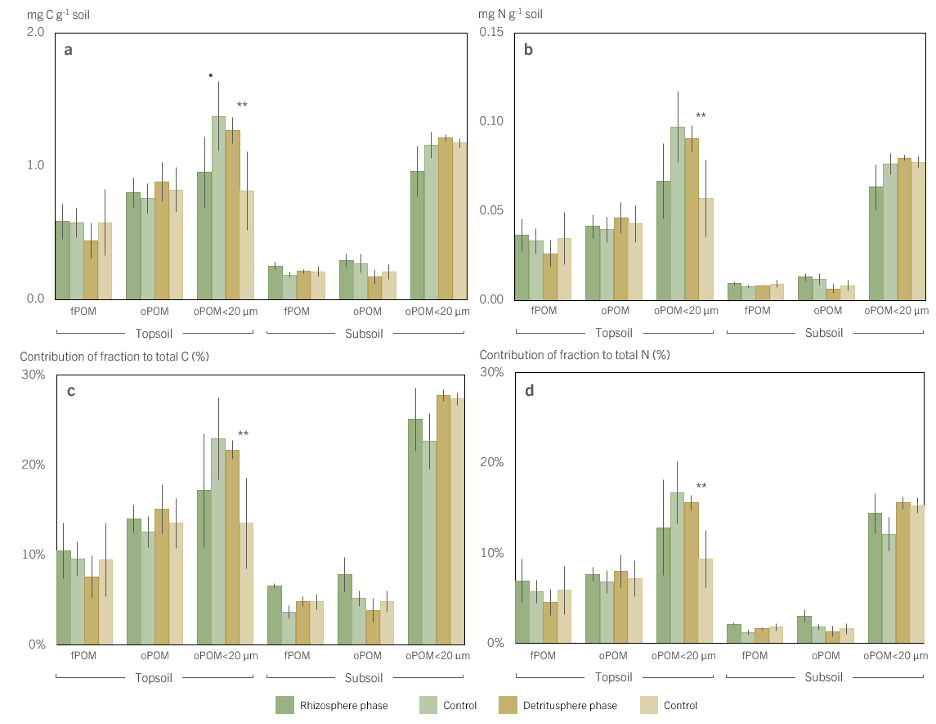
\includegraphics[width=1\textwidth]{img/M5-Figure_1.png}
	\caption{C and N contents in water-stable aggregate size classes. The contents of a) C and b) N (in \si{mg\,\gram^{-1}}\,fraction) in three water-stable aggregate-size classes and the concentrations of c) C and d) N (in \si{mg\,\gram^{-1}}\,soil) in the bulk soil. Green represents a living root phase (rhizosphere) and brown a decaying root phase (detritusphere) together with corresponding controls. Asterisks denote significant differences between rooted and control samples (\(.P < 0.1\), *\(P < 0.05\), **\(P < 0.01\), ***\(P < 0.001\)). Bars represent means \(\pm\)SD (\(n=6\) independent replicates).}
	\label{fig:M5-F1}
\end{figure}

Interestingly, contrary to the topsoil, the root effect was not isolated to macroaggregates in the subsoil, but also resulted in elevated C and N contents in larger microaggregates (\SIrange{53}{250}{\micro\metre}) compared to the corresponding controls (\num{5.49} in rooted samples and \SI{4.84}{mg\,C\,\gram^{-1}}\,soil in controls). In the topsoil, the effects of the living roots extended into the detritusphere phase in larger macroaggregates, with elevated C (\num{5.99} in rooted compared to \SI{5.27}{C\,\gram^{-1}} in controls, \(P=0.041\)) and N (\num{0.52} in rooted compared to \SI{0.45}{N\,\gram^{-1}} in controls, \(P=0.060\); Figure \ref{fig:M5-F1}c and Figure \ref{fig:M5-F1}d). This was not reflected in the subsoil.

\subsection{Elemental distribution in specific organic matter fractions}

Across treatments, the elemental compositions of the separated POM and MAOM fractions remained largely consistent, with almost no notable changes in their C and N contents around living or decaying roots.However, a clear change in the content of C and N (in \si{mg\,\gram^{-1}}\,soil) was observed in the oPOM<\SI{20}{\micro\metre} fraction within the topsoil (Figure \ref{fig:M5-F2}a and Figure \ref{fig:M5-F2}b). In the rhizosphere, the C content in oPOM<\SI{20}{\micro\metre} decreased slightly compared to unplanted controls (from \num{1.37} to \SI{0.95}{mg\,C\,\gram^{-1}}\,soil; \(P= 0.089\)). In the detritusphere, however, C in oPOM<\SI{20}{\micro\metre} was preserved around decaying roots compared to decreasing C contents of the same fractions in controls (\num{1.27} compared to \num{0.81}; \(P=0.025\); Figure \ref{fig:M5-F2}a and Figure \ref{fig:M5-F2}b). This was also reflected in the total amount of C allocated in oPOM<\SI{20}{\micro\metre} in the detritusphere (\num{38.07} compared to \SI{24.44}{mg\,C} in controls; \(P=0.052\)) and further emphasized by the maintained relative C and N contribution of the fraction around decaying roots in topsoil (Figure \ref{fig:M5-F2}c and Figure \ref{fig:M5-F2}d). This pattern was reversed around the living roots; although not significant, the total amount of C in oPOM<\SI{20}{\micro\metre} was slightly lower compared to the controls (\num{28.66} compared to \SI{41.30}{mg\,C}; \(P=0.187\)).

\begin{figure}[H]
	\centering
	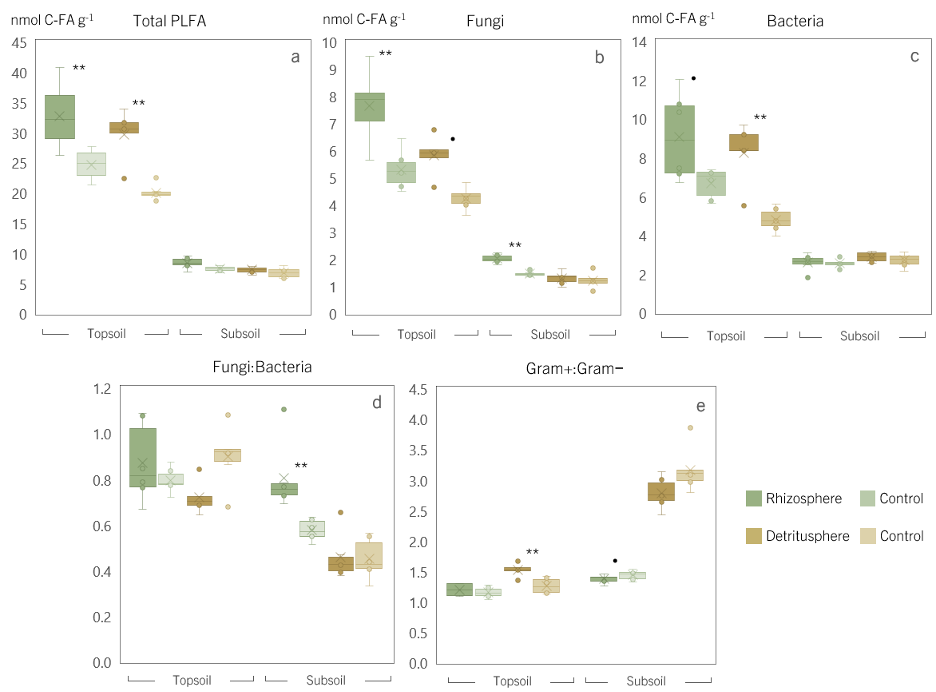
\includegraphics[width=1\textwidth]{img/M5-Figure_2.png}
	\caption{C and N contents in and contributions of particulate organic matter fractions. The content of a) C and b) N (in \si{mg\,\gram^{-1}}\,soil) and the contribution of c) C and d) N to the total stock (in \%) of organic matter fractions (fPOM, oPOM and oPOM<\SI{20}{\micro\metre}). Green represents a living root phase (rhizosphere) and brown a decaying root phase (detritusphere) together with corresponding controls in faded colors. Asterisks denote significant differences between rooted and control samples (\(.P < 0.1\), *\(P < 0.05\), **\(P < 0.01\), ***\(P < 0.001\)). Bars represent means \(\pm\)SD (\(n=3\) independent replicates).}
	\label{fig:M5-F2}
\end{figure}

The changes in the oPOM<\SI{20}{\micro\metre} fractions were not observed in the subsoil. Instead, there was a slight (non-significant) increase in the C contribution of the fPOM fraction in the subsoil rhizosphere (from \SI{3.63 \pm 0.74}{\percent} to \SI{6.59 \pm 0.27}{\percent}; \(P=0.154\); Figure \ref{fig:M5-F2}c). This led to increased C:N ratios of the fPOM fractions around living but also around decaying roots, from \num{24.37} to \num{26.88} in the rhizosphere (\(P=0.053\)) and from \num{22.91} to \num{25.36} in the detritusphere (\(P=0.086\)).

Although not significant, the fPOM fraction in the subsoil rhizosphere was further depleted in \textsuperscript{15}N (from \num{4.44} in controls to \SI{4.00}{\permil} in rooted samples; \(P < 0.001\)). In the detritusphere, this pattern was reversed, with the fraction instead enriched in \textsuperscript{15}N (from \num{4.26} in controls to \SI{4.77}{\permil} in rooted samples; \(P < 0.001\)). In MAOM fractions, we did not determine any significant changes in the isotopic composition across treatments. The chemical composition of the separated POM fractions (determined via \textsuperscript{13}C CP-MAS NMR) showed no differences between treatments, with little to no effect of the living or decaying roots. Further, the integrated regions showed similar chemical composition of the fractions, not only between the incubation phases, but also between the substrates.

\subsection{Phospholipid fatty acid analysis}

Microbially derived FAs increased in the rhizosphere of the topsoil substrate (from \num{24.62} to \SI{32.66}{nmol\,C\text{-}FA\,\gram^{-1}}\,soil; \(P=0.005\)) into the detritusphere phase, with the elevated microbial abundance being maintained in rooted topsoil samples compared to controls (\num{29.64} versus \SI{20.00}{nmol\,C\text{-}FA\,\gram^{-1}}\,soil; \(P=0.002\); Figure \ref{fig:M5-F3}a). Around living roots, both fungi and bacteria increased uniformly in the topsoil (Figure \ref{fig:M5-F3}b and Figure \ref{fig:M5-F3}c), as reflected by the fungi:bacteria ratio, which remained similar to controls despite the overall increase in FAs (Figure \ref{fig:M5-F3}d). However, as decomposition progressed, the fungal abundance around decaying roots decreased, while bacterial abundance was maintained. This was associated with a relative increase in Gram-positive bacteria around the decaying roots, as reflected in the elevated Gram+:Gram- ratio (from \num{0.70} to \num{0.90}; \(P=0.009\); Figure \ref{fig:M5-F3}e). In the subsoil, fungal abundance increased significantly around living roots compared to controls (\(P=0.007\)), similar to the differences observed in topsoil, with a shift in the fungi:bacteria ratio from \num{0.58} to \num{0.75} (\(P=0.005\)). During the detritusphere phase, no difference between roots and controls was observed in the subsoil.


\begin{figure}[H]
	\centering
	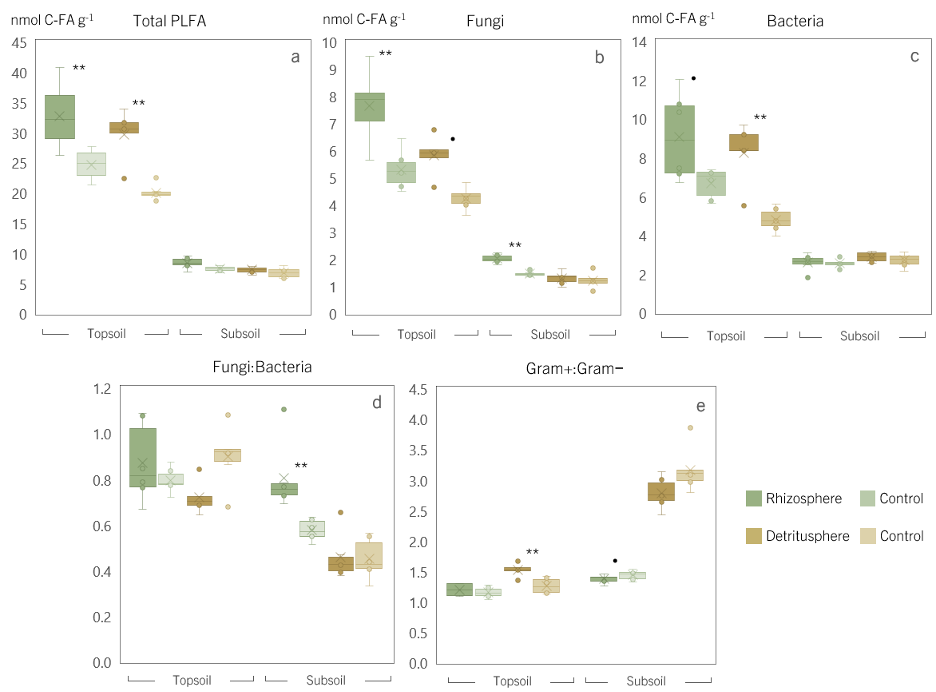
\includegraphics[width=1\textwidth]{img/M5-Figure_3.png}
	\caption{PLFA profiling of microbial community structure. The a) total content of extracted fatty acids (in \si{nmol\,C\text{-}FA\,\gram^{-1}}), the content of markers associated with b) fungi (\si{nmol\,C\text{-}FA\,\gram^{-1}}) and c) bacteria (\si{nmol\,C\text{-}FA\,\gram^{-1}}) and the d) fungi:bacteria ratio and e) Gram+:Gram− ratio in a topsoil and subsoil. Green boxes represent the living root phase (rhizosphere) and brown the decaying root phase (detritusphere) together with corresponding controls in faded colors. Asterisks denote significant differences between rooted and control samples (\(.P < 0.1\), *\(P < 0.05\), **\(P < 0.01\), ***\(P < 0.001\)). Box plots indicate medians (line) and means (x), where the first (Q1) and third (Q3) quartile are represented by the lower, respectively upper bounds of the box. Error bars represent the data range, bounded to \(1.5 \times (\text{Q3}-\text{Q1})\); (\(n = 6\) independent replicates).}
	\label{fig:M5-F3}
\end{figure}

\section{Discussion}

The purpose of this study was to investigate how plant roots drive soil structure formation and SOM build-up during early stages of soil development in a dryland soil system. The experiment was designed to follow the natural undisturbed succession from rhizosphere to detritusphere, aiming at capturing possible legacy effects from the rhizosphere influencing the development of the detritusphere. This allowed for the direct observation of changes in SOM formation, aggregation, and microbial community composition during phases where C inputs were primarily derived from either active rhizodeposition ('rhizosphere phase') or decaying root litter inputs ('detritusphere phase'). We hereby demonstrate how root-microbe-soil interactions change during the transition from rhizosphere to detritusphere, and how these processes are partially constrained—or counterbalanced—depending on the soil substrate in which the roots grow and later decompose.

\subsection{The rhizosphere: rhizodeposition as C input}

In the studied dryland soil, roots induced a shift in soil aggregation in the rhizosphere, leading to an increased contribution of water-stable macroaggregates to the total mass and an increased allocation of C and N to macroaggregates in both topsoil and subsoil (Figure \ref{fig:M5-F1}c and Figure \ref{fig:M5-F4}d; Figure \ref{fig:figure_4a_label}). This root effect is consistent with the well-established consensus that plant roots drive the formation of coarser aggregate structures, for example via root-derived gluing agents or direct entanglement of soil particles \citep{Tisdall1982, Six2004, Angst2018, Gregory2022}.

\begin{figure}[H]
	\centering
	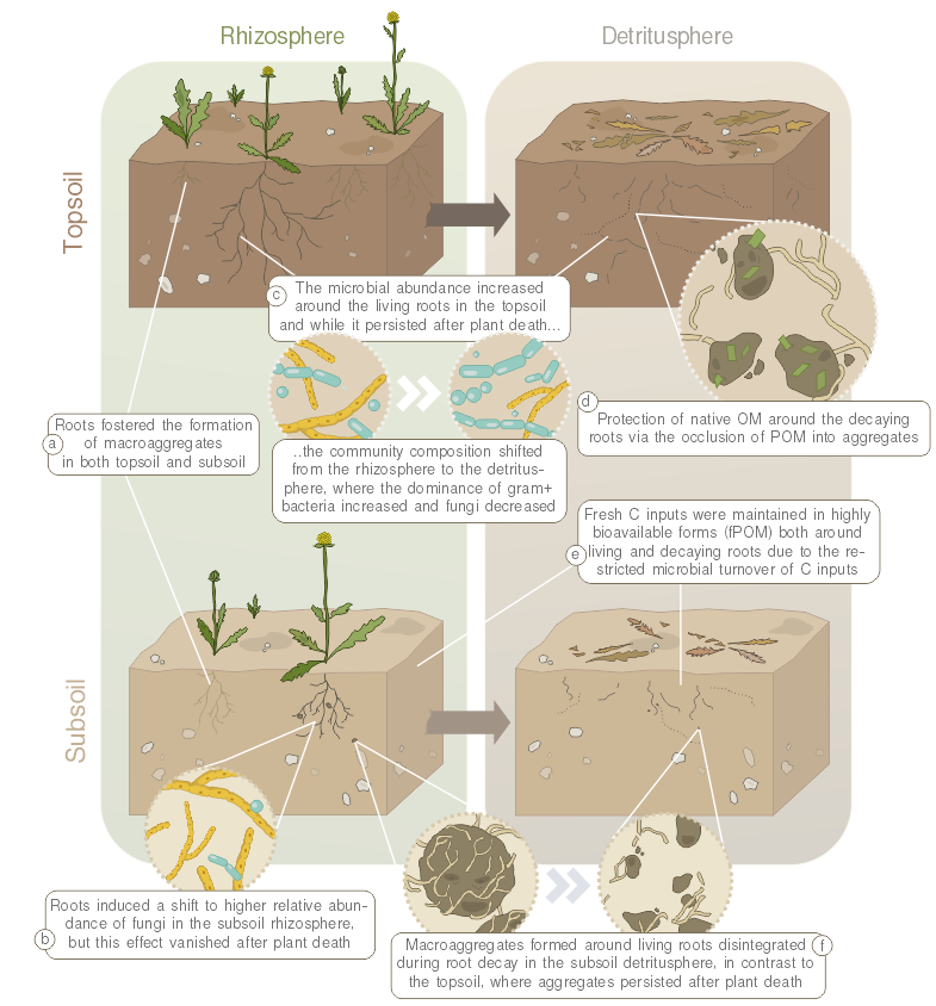
\includegraphics[width=1\textwidth]{img/M5-Figure_4.png}
	\caption{a) Living roots fostered the formation of macroaggregates in both topsoil and subsoil, and b) induced a change in the microbial community composition in the subsoil towards a higher relative abundance of fungi. This was not reflected in the topsoil, where c) the microbial abundance instead increased uniformly in the rhizosphere without structural changes in the community. While the increased total microbial abundance was maintained in the detritusphere, the composition changed as Gram+ bacteria outcompeted fungi. Around decaying roots in the topsoil, d) OM was protected in aggregates via the formation of occluded POM (oPOM<\SI{20}{\micro\metre}) and in the subsoil, e) the slower microbial C turnover resulted in an accumulation of fresh C inputs in highly bioavailable forms (fPOM) around both living and decaying roots. While the root-induced macroaggregates persisted after plant death in the topsoil, f) the aggregates disintegrated in the subsoil around the decaying roots.}
	\label{fig:M5-F4}
\end{figure}

The pioneer plant shaped the composition of the microbial community around the living roots. Driven by the easily available OM from the rhizodeposits, the total microbial abundance increased significantly in the topsoil rhizosphere (Figure \ref{fig:M5-F3}a). Interestingly, both fungi and bacteria increased similarly (Figure \ref{fig:M5-F3}b and Figure \ref{fig:M5-F3}c), meaning that the overall community structure remained unaffected by rooting (Figure \ref{fig:M5-F4}c). In contrast, there was no substantial increase in total microbial abundance in the subsoil rhizosphere. Instead, we determine a pronounced community shift towards a higher relative abundance of fungi in the subsoil (Figure \ref{fig:M5-F3}b), while bacterial abundance remained unaffected by the roots (Figure \ref{fig:M5-F4}b). These findings are in accordance with the widely accepted notion that conditions in the rhizosphere favor fungi over other microbial groups \citep{Butler2003, Brant2006, Denef2009}. This could be due to the lower content and diversity of SOM (including native OM) in the subsoil, where the filamentous growth of the fungal mycelium benefit fungi in gaining access to heterogeneously distributed OM resources, compared to bacteria with rather restricted motility in the soil \citep{DeBoer2005}.

Roots grown in the subsoil were of lower litter quality (higher lignin\textsubscript{NMR}:N ratio) compared to in the topsoil, and as fungi are adapted to assimilate more complex C resources from litter, this may have further amplified the distinction of fungi in the subsoil \citep{Poll2006}. Moreover, it is possible that this shift towards increased fungal dominance in the subsoil contributes not only to root-induced macroaggregation, but also to the observed microaggregation in the subsoil rhizosphere, which was not observed in the topsoil (Figure \ref{fig:M5-F1}a and Figure \ref{fig:M5-F1}b). Fungal hyphae as vectors for macroaggregation have been widely reported (e.g., \citeauthor{Bossuyt2001}, \citeyear{Bossuyt2001}; \citeauthor{Lehmann2020}, \citeyear{Lehmann2020}; \citeauthor{Bucka2021}, \citeyear{Bucka2021}), but evidence for the processes associated with fungal-induced microaggregation remains scarce. \citet{Vidal2018} show how hyphae are in fact closely linked to soil microstructure formation directly at the root-soil interface. \citet{Rillig2006} further point to mycorrhizal fungal mycelial products as drivers of the formation of smaller aggregates. As arbuscular mycorrhizal colonization has been reported for the pioneer species used in this study growing in adjacent study sites (\textit{Helenium aromaticum}; \citeauthor{Dhillion1995}, \citeyear{Dhillion1995}), mycelial byproducts and mutualistic plant-microbial interactions may be a contributing factor to the increased microaggregation in the subsoil. The increased fungal abundance in the subsoil rhizosphere is consistent with the findings of \citet{Baumert2021} and overall emphasizes fungi as key players in the assimilation of root-derived C compounds in the subsoil.

In association with the increased fungal dominance in the subsoil rhizosphere, we determine that the effect of the roots on aggregation was not isolated to macroaggregates in the subsoil but extended to larger microaggregates, where C and N contents were elevated compared to the controls (Figure \ref{fig:M5-F1}a and Figure \ref{fig:M5-F1}b), which further highlights the importance of labile root-derived gluing agents for aggregate formation during early rhizosphere development in C poor subsoils \citep{Baumert2018}.

\subsection{The detritusphere: root litter as C input}

After plant death, as the rhizosphere transitioned to a detritusphere, the initially formed root-induced macroaggregation remained in the topsoil but entirely disintegrated in the subsoil. The overall lack of aggregate stability over time is consistent with observations showing that a continuous input of OM is necessary to maintain aggregate structures, and that the disintegration of macroaggregates begins during early stages of decomposition when available C sources and microbial activity decline (e.g., \citeauthor{Golchin1997}, \citeyear{Golchin1997}; \citeauthor{Helfrich2008}, \citeyear{Helfrich2008}). In the present study, disintegration of newly formed aggregates was indeed particularly pronounced in the C poor subsoil (Figure \ref{fig:M5-F4}f), which is supported by the work of \citet{Bucka2021}, who report low mechanical stability of newly formed macroaggregates after OM addition in initial soils compared to greater retained aggregate stability in mature soils \citep{Felde2020}. This suggests that aggregates initially formed in the rhizosphere are only loosely connected, and that a living root system---or continuous C input---is a prerequisite for aggregate formation and persistence in soil systems with otherwise limited C inputs. Furthermore, these results suggest that a certain 'backbone' of native C, as in the topsoil, is required for long-term aggregate stabilization in arid soil systems. The difference between topsoil and subsoil may have been further amplified by the fact that roots grown in subsoil had lower litter quality (higher C:N and lignin\textsubscript{NMR}:N ratio; Table \ref{tab:M5-T1}; \citeauthor{Walela2014}, \citeyear{Walela2014}) compared to those grown in topsoil, further reinforcing the limiting conditions for microbial activity.

The transition from a living to a decaying root system, and thereby from C inputs dominated by low molecular weight compounds to more complex structural litter-derived C sources, shaped the composition and structure of the microbial community. The relative dominance of Gram+ over Gram- bacteria increased distinctively in the detritusphere of both soil substrates (Figure \ref{fig:M5-F3}e). This was likely driven by the increasing complexity of the litter resources as the decomposition progressed (e.g., as indicated by increasing (Ac/Al)\textsubscript{V} ratios; Table \ref{tab:M5-T1}), favoring Gram+ bacteria which are specialized in the processing of complex C sources \citep{Fanin2019, Denef2009, Butler2003}. This is supported by \citet{Shi2018}, who show how the microbial genetic potential to decompose complex macromolecular compounds increases in the absence of living roots, while root exudates in the rhizosphere instead promote the development of a microbial community with increased capacity to utilize low molecular weight compounds. This underscores how the presence of living and decaying roots modulates litter decomposition through alterations in microbial functionality. Furthermore, \citet{Nuccio2020} specifically describe how both temporal and spatial niche microbial coexistence is fostered in the combined rhizosphere-detritusphere, which opens up important future research opportunities in the transition zone from rhizosphere to detritusphere and highlights need for further research including microbial functional traits.

Interestingly, the shift in the microbiome around decaying roots in the topsoil was not associated with a change in overall abundance---in fact, abundance prevailed from the rhizosphere to the detritusphere phase, while decreasing in the corresponding controls (Figure \ref{fig:M5-F3}a). Consequently, despite the resource-limited conditions as decomposition progressed, litter-derived C inputs were sufficient to maintain microbial abundance, but the conditions favored those microbial groups specialized in utilizing complex C sources.

Another shift in microbial community structure in the detritusphere was observed in fungi, where both total fungal abundance and relative abundance to bacteria decreased, particularly so in the subsoil (Figure \ref{fig:M5-F3}b and Figure \ref{fig:M5-F3}d). The shift towards bacterial dominance in the detritusphere contrasts with the general notion of fungi as key players in litter decomposition \citep{Williams2006, Voriskova2013}. As PLFA profiles were only quantified at one point during the decomposition process in the present study, this represents only a snapshot of the ongoing succession of the microbial community involved in decomposition. \citet{Herman2012} found that fungal dominance during litter decomposition decreased rapidly after 21 days, after which Gram+ and Gram- increased. \citet{Voriskova2013} further emphasized the succession of the fungal community during decomposition, with different fungal taxa being highly abundant only during short periods. Thus, our results do not necessarily exclude fungal involvement in the initial stages of litter decomposition, but rather point to the increasing importance of bacteria during the late stages of decomposition, when labile litter components are depleted. This is supported by \citet{Esperschuetz2011} showing how Gram+ outcompete fungi in litter degradation in resource-limited systems where N is scarce. The retreat of fungi in the developed detritusphere in subsoil equates to the loss of the hyphal networks that enmeshed soil particles, which may cause the disintegration of aggregates around the decaying roots. This underlines the direct involvement of hyphae as a temporary binding agent in the rhizosphere that does not persist into the detritusphere \citep{Six2004}.

\subsection{Elemental composition of rhizosphere and detritusphere}

Contrary to our hypothesis, roots had no notable effects on total C and N contents in the bulk soil in the rhizosphere in either of the two soil substrates. It is possible that root inputs to the system were minor in comparison with other soil C pools, or that the inputs were rapidly processed by the stimulated microbial activity in the vicinity of the roots. Given the enhanced microbial abundance and changed community composition around the roots (Figure \ref{fig:M5-F3}), the second option appeared to be more likely. Nevertheless, it should be noted that the entire, thoroughly rooted pot was considered as 'rhizosphere' in the present study. Indeed, there is no clear definition of the spatial extent of the rhizosphere or where the boundaries of the rhizosphere are, as it depends on the parameters studied \citep{Kuzyakov2019}. However, most root-driven processes are concentrated in the immediate soil volume around the roots and diluted in the surrounding soil. For example, microbial abundance has been shown to be concentrated in the first \SIrange{1}{2}{\milli\metre} around the roots \citep{Marschner2012}, and rhizodeposits may have restricted dispersal potential from the immediate soil volume around the roots \citep{Kuzyakov2019}. This means that certain root effects may have been overseen, or diluted, given the large soil volume representing the rhizosphere. Under these circumstances, \textsuperscript{13}C labeling of the pioneer plants might have facilitated the quantification of small-scale elemental changes, thereby allowing a more detailed understanding of the fate of root-derived C in the soil, both in the rhizosphere and the subsequent detritusphere \citep{Teixeira2024}.

\subsection{Changes in POM around living and decaying roots}

Surprisingly, neither living nor decaying roots affected the composition of POM and MAOM, as evidenced by consistent C and N contents and comparable chemical compositions in all fractions. In the topsoil, however, occluded C as oPOM<\SI{20}{\micro\metre} and the contribution of this fraction to total C and N were clearly affected---albeit in contrasting ways between the rhizosphere and the detritusphere (Figure \ref{fig:M5-F2}). In the soil around the living root system, a slight decrease in occluded C was observed compared to the control, suggesting increased aggregate turnover around the roots \citep{Wang2020}. Root-induced breakdown of aggregates, combined with stimulated microbial activity around the roots resulting in an enhanced rhizosphere priming effect, could be contributing factors to the release and ultimate loss of bioavailable POM in the rhizosphere \citep{Cheng2009}. Around the decaying roots, the pattern was reversed, where instead an accumulation of occluded C (oPOM<\SI{20}{\micro\metre}) was determined (Figure \ref{fig:M5-F4}d). This highlights decaying roots as a prerequisite for the formation of occluded POM and shows how decaying litter surfaces in the detritusphere represent functional components that facilitate aggregate formation, directly contributing to the long-term stabilization of organic C in the soil \citep{Witzgall2021}.

In the subsoil, we observed elevated C:N ratios in the fPOM fractions in both the rhizosphere and detritusphere compared to unplanted controls Figure \ref{fig:M5-F4}e). During the rhizosphere phase, this was further associated with \textsuperscript{15}N depletion, indicating fresh C inputs into the fraction, as the opposite---increasing aliphaticity of OM---would otherwise lead to \textsuperscript{15}N accumulation \citep{Kramer2003}. This means that fresh C inputs remained in highly bioavailable forms (i.e., not occluded into aggregates or associated with mineral surfaces) and did not undergo notable microbial transformation during the course of both incubation phases. This phenomenon was only observed in subsoil, as there was no evidence of fresh C inputs in the fPOM fraction in the topsoil. This difference between the soil substrates can be attributed to restricted microbial abundance in the subsoil, resulting in slower C turnover compared to the topsoil where labile inputs were rapidly transformed. This may, in part, be related to the chemistry of the plant tissue in the subsoil, where roots were of lower biochemical quality compared to those in the topsoil (broader C:N ratios and elevated lignin\textsubscript{NMR}:N ratios; Table \ref{tab:M5-T1}; \citeauthor{Walela2014}, \citeyear{Walela2014}). These findings highlight the limiting conditions for microbial activity and suggest that lower quality litter is less preferred as a nutrient source for microbial decomposers. Collectively, these observations underscore the importance of roots as a critical source of POM in dryland subsoils, with legacy effects that can persist even after plant death \citep{Angst2016}. Furthermore, they emphasize how the litter chemistry of OM inputs shapes microbial community composition, with implications for aggregate formation.

\section{Conclusion}

In this study, we explore the interaction between plant roots, microorganisms, and soil during the succession from a rhizosphere to a root detritusphere in a dryland topsoil and subsoil. Our results highlight the fundamental role of roots in driving soil structure formation, microbial succession, and OM formation during the early stages of soil development. While we found root-induced macroaggregation in the topsoil, the effect of roots was extended to both increased macro- and micro-aggregates in the subsoil, presumably facilitated by fungal hyphae in the subsoil rhizosphere. However, with plant death, as the rhizosphere transitioned to a detritusphere, the newly formed aggregates disintegrated in the subsoil, underscoring the critical importance of continuous OM inputs for maintaining more persistent aggregate structures in C-poor subsoils. The transition to a detritusphere was further associated with a clear decline in fungal abundance and an increased dominance of Gram+ bacteria, emphasizing their role in mineralizing increasingly complex C resources in the developing detritusphere in dryland soils. Conversely, we found legacy effects of living roots imprinted in the topsoil, as macroaggregates formed within the rhizosphere persisted after plant death, and the microbiome developed around living roots was maintained in the detritusphere. While we found no changes in MAOM around the roots, we highlight the build-up of occluded POM facilitated by decaying root litter in the topsoil, underscoring the influence of root residues on SOM formation and persistence within the root detritusphere. Our work thus highlights the intricate interactions of plants, microorganisms, and soil particles in the vicinity of living and decaying roots in dryland soil systems, and how the biogeochemical processes involved are regulated by the soil substrate in which the roots grow and decompose. Our results further underscore the importance of encompassing the \textit{in situ} transition from living to decaying roots to advance our understanding of the dynamics of the legacy from rhizosphere and detritusphere.

\section*{CRediT authorship contribution statement}

\begin{description}
    \item[K. Witzgall:] Writing- review \& editing, Writing- original draft, Visualization, Methodology, Investigation, Formal analysis, Data curation, Conceptualization.
    \item[F.A. Steiner:] Writing- review \& editing, Writing- original draft, Investigation, Formal analysis, Data curation, Conceptualization.
    \item[B.D. Hesse:] Writing- review \& editing, Investigation, Data curation.
    \item[N. Riveras-Mu{\~n}oz:] Writing- review \& editing, Methodology, Data curation.
    \item[V. Rodr{\'\i}guez:] Writing- review \& editing, Methodology, Data curation. % Assuming accent on i
    \item[P.P.C. Teixeira:] Writing- review \& editing, Validation, Investigation.
    \item[M. Li:] Methodology.
    \item[R. Oses:] Writing- review \& editing, Conceptualization.
    \item[O. Seguel:] Writing- review \& editing, Conceptualization.
    \item[S. Seitz:] Writing- review \& editing, Conceptualization.
    \item[D. Wagner:] Writing- review \& editing, Supervision, Conceptualization.
    \item[T. Scholten:] Writing- review \& editing, Supervision, Resources, Funding acquisition, Conceptualization.
    \item[F. Buegger:] Writing- review \& editing, Formal analysis, Data curation.
    \item[G. Angst:] Writing- review \& editing, Supervision, Data curation, Conceptualization.
    \item[C.W. Mueller:] Writing- review \& editing, Validation, Supervision, Project administration, Methodology, Funding acquisition, Conceptualization.
\end{description}

\section*{Declaration of competing interest}

The authors declare that they have no known competing financial interests or personal relationships that could influence the work reported in this paper.

\section*{Data availability}

Data will be made available on request.

\section*{Acknowledgements}

The authors are grateful for the help and support of Maria Greiner and Nina Meschnark who supported the laboratory analyses. 
We also thank Josef Reischenbeck who built the machine used for aggregate fractionation. This work was financially supported by the German Research Foundation (DFG) as part of the 'EarthShape' priority program [grant no. MU3021/6-2; \url{www.earthshape.net}].

\section*{Supplementary data}

Supplementary data to this article can be found online at \url{https://doi.org/10.1016/j.soilbio.2024.109503}.

\bibliographystyle{natbib}
\bibliography{literatur-M5}
